%
%
%
\long\def\comment#1{}
\newif\ifcover

% \documentstyle[times,chi2003ea]{article}
% \documentclass[nocopyrightspace,times]{chiproceedings-nospace}
% \documentclass[nocopyrightspace]{chiproceedings-nospace}

% パタンはtt
% 出力文字列はsf

\documentclass{article}
\usepackage{times}
\usepackage{uist04}

\usepackage{here} % [H]とするとその場所に配置されるらしい

\long\def\ttt#1{\texttt{\small #1}}
\long\def\tsf#1{\textsf{\small{#1}}}
\long\def\tit#1{\textit{\small{#1}}}

\usepackage{graphicx}
% mediabb.sty というのを使うとPDFをそのままincludegraphicsできるらしい。
% http://www.ns.musashi-tech.ac.jp/~inoue/Pages/TeX/mediabb.sty.html
%
% \usepackage{mediabb}
% \usepackage{ascmac}

\begin{document}
\title{Strotor: A Minimalistic Approach to \\
Exploring Large Hierarchical Data}
\author{
\begin{tabular}{l}
\parbox{5.5cm}{
\begin{center}
Toshiyuki Masui\\
Keio University\\
masui@pitecan.com
~ \\
~ \\
~
\end{center}
}
\end{tabular}
}
\maketitle
\abstract
We introduce a new simple information navigation technique
that enables users to explore large hierarchical data structure
using only two keys or one rotating device that can generate
two different signals based on the rotation direction.
%
Using the disk-based system called "Strotor",
users can find an entry in a huge hierarchical database easily
only by rotating a disk or a cylinder in two directions.
%
Strotor can be easily installed in sofas, kitchens, cars, etc.
where standard keyboards and remote controllers do not fit.

\keywords Help systems, Approximate pattern matching, Generate-and-filter

\tolerance=400 
  % makes some lines with lots of white space, but 	
  % tends to prevent words from sticking out in the margin

\section*{INTRODUCTION}

Huge data are often represented as a hierarchical data structure, and
various navigation methods are provided for exploring the data.
For example, files on Unix are structured hierarchically, and
various commands (\tsf{cd}, \tsf{ls}, etc.) and APIs are provided for exploring the file system.
Large dictionary database can also be treated as a large
hierarchical data, since the name of the entry can be treated hierarchically:
e.g. an entry for ``dictionary'' can be stored under ``d'' and ``d/i''.

Many information visualization techniques and navigation techniques for huge hierarchical data
have been proposed.
On personal computers,
multiple GUI methods are provided for
exploring the hierarchical file structure, because
there is no best interaction technique for all the users and situations.
% there is no single interaction technique that is always good for any situation.

When a user cannot use a pointing device or a standard keyboard,
selection-based interaction techniques are used for
finding information in hierarchical data.
For example, a user can hierarchically find a music file by
selecting an artist from the list of artist names,
selecting an album title from the title list,
and selecting a music file from the song list.
% Users can do the selection jobs either by using a mouse or by using arrow keys.
% For exaple,
Users can use two keys for choosing an entry from the list
(e.g. selecting an artist from the artist list),
and another key is used for selecting an entry and show the next level
(e.g. selecting an artist and show album titles).
It is also necessary to provide a way to go back to the previous state, and
another key can be used for that task
(e.g. showing the artist list for artist selection).
%
This 4-way navigation is popular on small mp3 players\footnote{
  e.g. http://www.iriver.com/product/view.asp?pCode=003\&pNo=37
} and remote controllers like AppleRemote\footnote{http://en.wikipedia.org/wiki/Apple\_Remote}
for selecting a song from the hierarchical data.
4-way navigation is also available on desktop software like Finder.app on Mac.

\begin{figure}[H]
\centerline{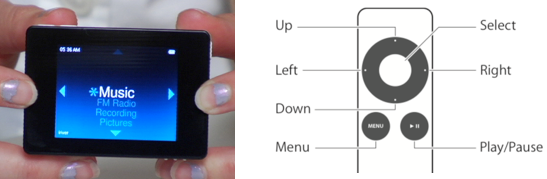
\includegraphics[width=80mm,bb=0 0 547 179]{figures/4buttons.png}}
\caption{4-button controllers on a small mp3 player and AppleRemote.}
\label{u10}
\end{figure}

% http://www.reigncom.com/eng/media/press/en_pr_read.asp?no_noti=1630&cd_noti_host=9
% D-Click Control System

% Small devices like Rio MP3 player and remote controllers like AppleRemote have
% 4 buttons for selecting a song from the hierarchical data.

Using 4 keys might be okay on these devices, but it would be much better
if we could do the navigation task using only 2 keys.
In that case, we can use a rotating device like a disk or a cylinder for the navigation,
since the device can generate two key signals based on the direction of the rotation.
%
We have developed a new navigation technique where only two keys are required
for exploring large hierarchical data, and implemented the system on
a rotating device ``Strotor''.

% (語源)
% Navigating large structured data through rotation.

\section*{Navigation Method and Examples}

Stroter's behavior is based on the following simple principles:

\begin{enumerate}
\item Display the selected element, its siblings, its ancestors and their siblings,
and highlight the selected element.
\item If the selected element has children, wait for a little moment,
select the first child, and perform 1.
As a result, all the siblings of the newly selected element appear in the list.
\item When a user types U or D, select the element that is displayed next to the currently
selected element and perform 1.
If the depth of the newly selected element is different from the currently
selected element, siblings of the currently selected element will disappear.
\end{enumerate}

We will show how these works, using a hierarchical data structure of
shops in a shopping mall shown in Figure 1.
Rectangles with thick border represent categories, and
other rectangles represent individual shops.
We use two keys, "U" (up key) and "D" (down key), for the navigation.

\begin{figure}[H]
% 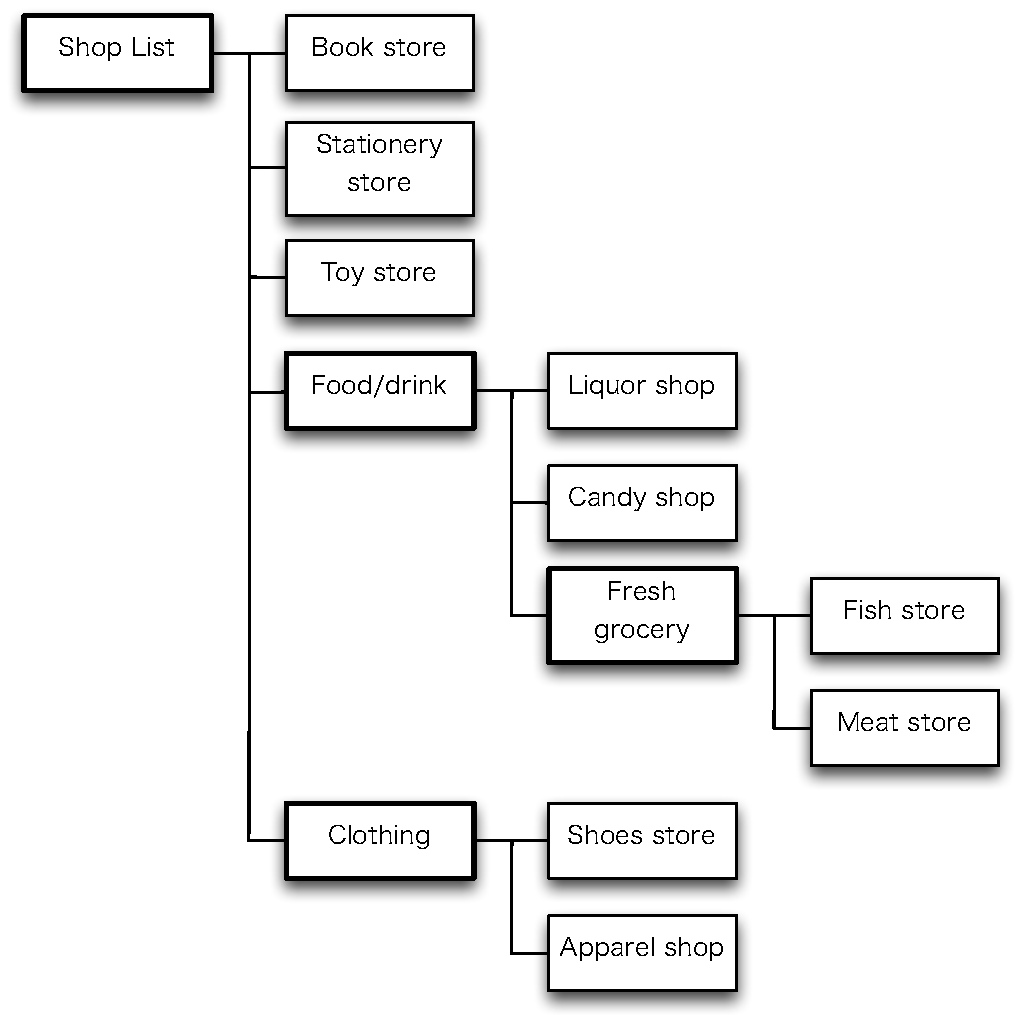
\includegraphics[width=70mm]{figures/fig1.pdf}
\centerline{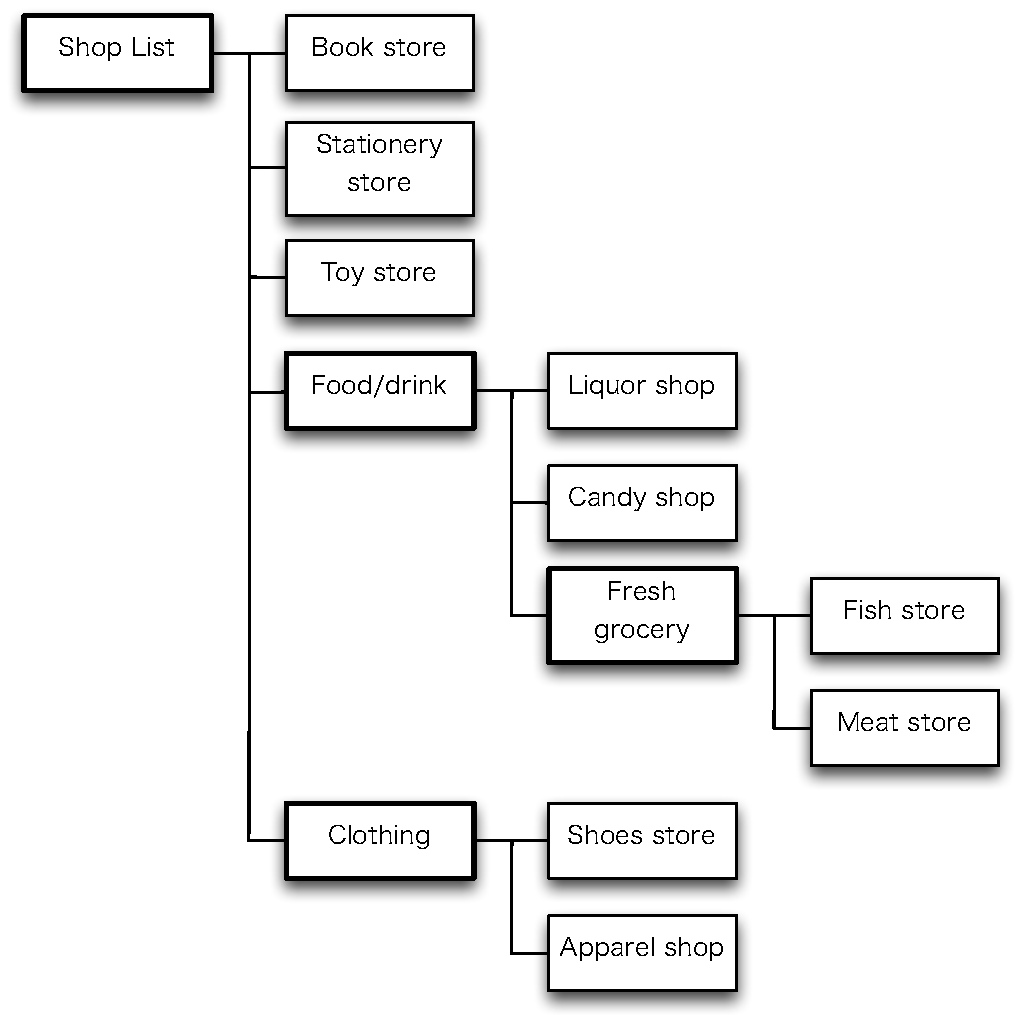
\includegraphics[width=70mm,bb=0 0 490 490]{figures/fig1.pdf}}
\caption{Shops in a shopping mall.}
\label{fig1}
\end{figure}

When the system starts, only the shops and categories
at the top level are displayed (Figure 2).
When the user types D,
the second element (Stationery store) is selected (Figure 3).

\begin{figure}[H]
\centerline{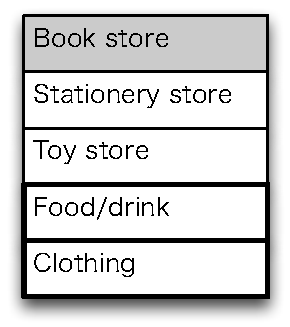
\includegraphics[width=24mm,bb=0 0 139 157]{figures/fig2.pdf}}
\caption{Initial display.}
\label{fig2}
\end{figure}

\begin{figure}[H]
\centerline{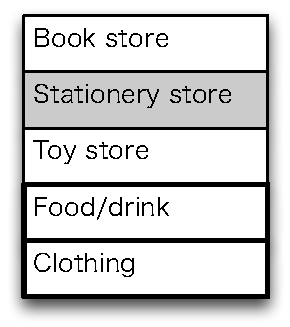
\includegraphics[width=24mm,bb=0 0 139 157]{figures/fig3.pdf}}
\caption{Initial display.}
\label{fig3}
\end{figure}

If the user types D two more times, 
\tsf{Food/drink} category is selected (Figure 4).
If the user stops typing keys and waits for a moment, the shops under the \tsf{Food/drink}
category are displayed, and the first entry (\tsf{Liquor shop}) is automatically selected (Figure 5).

\begin{figure}[H]
\centerline{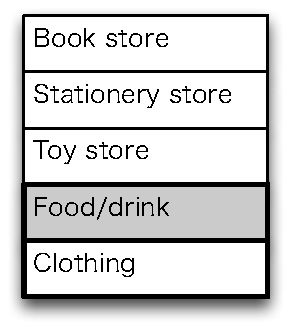
\includegraphics[width=24mm,bb=0 0 139 157]{figures/fig4.pdf}}
\caption{Initial display.}
\label{fig4}
\end{figure}

\begin{figure}[H]
\centerline{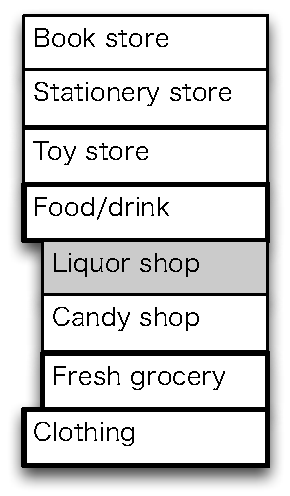
\includegraphics[width=24mm,bb=0 0 139 238]{figures/fig5.pdf}}
\caption{Initial display.}
\label{fig5}
\end{figure}

When the user types D twice and stops typing,
\tsf{Fresh grocery} category is selected (Figure 6), and
the shops under the category is automatically selected (Figure 7).

\begin{figure}[H]
\centerline{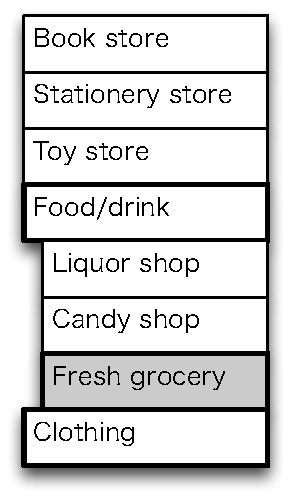
\includegraphics[width=24mm,bb=0 0 139 238]{figures/fig6.pdf}}
\caption{Initial display.}
\label{fig6}
\end{figure}

\begin{figure}[H]
\centerline{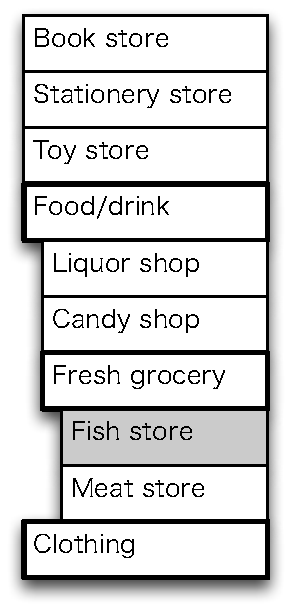
\includegraphics[width=24mm,bb=0 0 139 292]{figures/fig7.pdf}}
\caption{Initial display.}
\label{fig7}
\end{figure}

When the user types U here, \tsf{Fresh grocery} is selected,
the shops under \tsf{Fresh grocery} disappears (Figure 6).
If the user types U two more times, the display changes to Figure 5,
and one more typing U will generate? Figure 4.

If the user types D in Figure 4, the next visible entry
(\tsf{Clothing}) is selected (Figure 8), and then change to Figure 9.

\begin{figure}[H]
\centerline{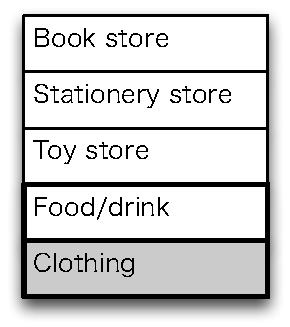
\includegraphics[width=24mm,bb=0 0 139 157]{figures/fig8.pdf}}
\caption{Initial display.}
\label{fig8}
\end{figure}

\begin{figure}[H]
\centerline{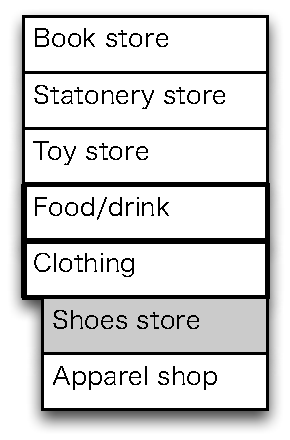
\includegraphics[width=24mm,bb=0 0 139 211]{figures/fig9.pdf}}
\caption{Initial display.}
\label{fig9}
\end{figure}

When the user types D twice in Figure 7,
\tsf{Clothing} is selected, and Figure 8 appears.

In this way, users can navigate through the hierarchical structure
only by typing U/D keys at the right timing.

\section*{Implementation}

A prototype system was built in JavaScript and the system runs on modern browsers.
Huge list of of news articles, movies, anime films, musics, and e-books are listed in one browser window
and the content is displayed in another window.
Users can hit two arrow keys or use the PowerMate device for the navigation.

\section*{DISCUSSIONS}

\subsection{Comparison with existing methods}

4-way navigation are quite common for exploring hierarchical data structure,
and modern computer users have no problem using it.
Many mobile phones and PDAs are equipped with a jog dial with a push button,
where the dial is used for selecting an item from a list and 
the push button is used for moving to the next level.
PowerMate is equipped with a push button which can used for such purposes.
As far as we know,
Strotor is the only interaction method for exploring hierarchical data structure
with only two keys or one rotating device.

Using a conventional hierarchical menu, children elements are displayed automatically
when the parent element is selected by a mouse.
The ``automatic expansion'' feature is Strotorと同じ。

\subsection{Comparison with InfoVis techniques}

Various information techniques like
Treemap\cite{Johnson:1991:TSA:949607.949654},
Hyperbolic Tree\cite{Lamping:1995:FTB:223904.223956},
and Sunburst\cite{Stasko:2000:FDN:857190.857683}
have been proposed for visualizing large hierarchical data.
Zooming interface (ZUI) systems like Pad[], Pad++[]
have also been used for handling ...
All of these systems are useful for understanding the structure of
large hierarchical data, but users of these systems have to use a pointing device
for exploring the whole data.

LensBar\cite{Masui:1998:LVB:647341.721215}
is also a ZUI system for handling large hierarchical data,
but the same data structure used in LensBar can be used for Strotor.
Users can use a pointing devices when it is appropriate,
and use two keys or a disk device when pointing devices is not available.

時間を使っているのは問題
可逆的でないから

\subsection{Subjective Evaluations}

No formal evaluation have been done yet, but Strotor has been used in the authors'
living room for several months, and the author's family members are using it
everyday for watching anime films and listening to music.

Since the only thing a user can do with Strotor is rotating the device,
a user can use the device and see what happens without thinking about
other interactions.
Using a disk device for data navigation might be a new experience for
most of the users, but the hard restriction of the usage seems to be a
good thing.

Selecting a content only by rotating a dial is very 気持ち良い。

% 音楽ソース、ニュースソース、動画、Wikipediaなどあらゆるものをダイヤルやペダルだけで検索できる

\section*{CONCLUSIONS}


\bibliographystyle{plain}
\bibliography{paper}

\end{document}


